\begin{figure}[!h]
	\begin{minipage}[b]{1.0\linewidth}
		\centering
		\centerline{ 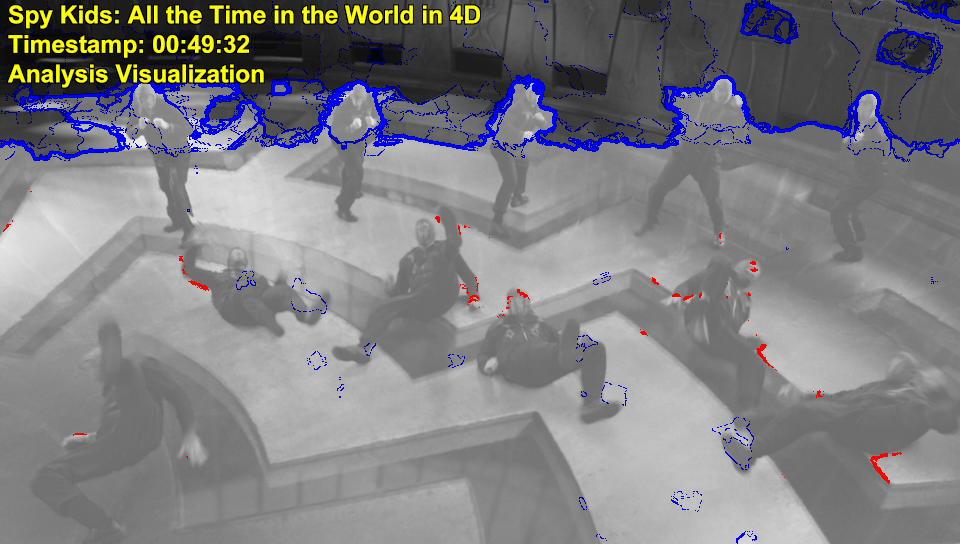
\includegraphics[width=0.8\textwidth]{example_spy} }
	\end{minipage}
	\begin{minipage}[b]{1.0\linewidth}
		\centering
		\centerline{ 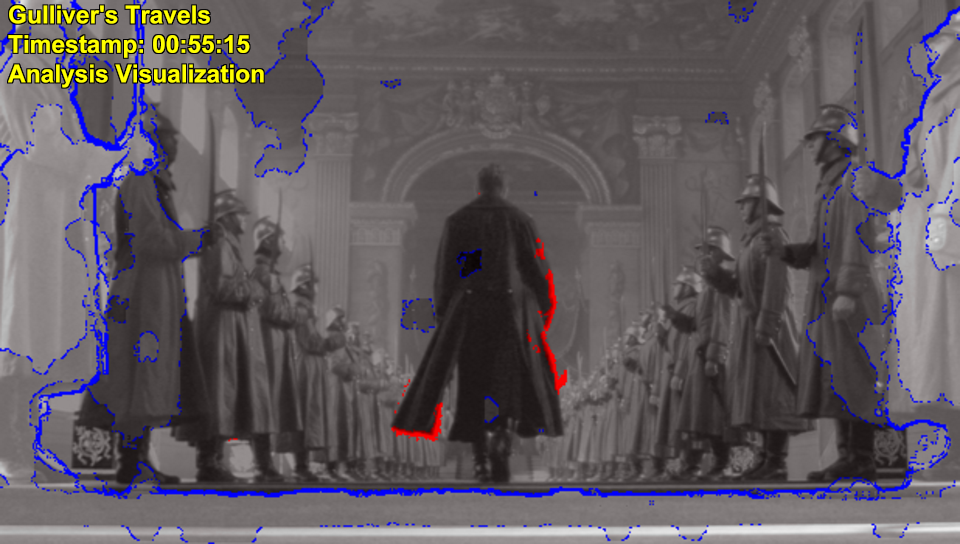
\includegraphics[width=0.8\textwidth]{example_gulliver} }
	\end{minipage}
    \caption{Пример результатов срабатвания алгоритма. В данных сценах
    	объекты переднего плана <<слиты>> с фоном. Для наглядности
    	поверх исходного кадра изображены карта диспаратности, границы
    	карты диспаратности (синие), и границы объектов, которые алгоритм посчитал
    	потерянными (красные).}
	\label{fig:res_example}
\end{figure}
